\documentclass{article}

\usepackage{graphicx}
\usepackage{tikz}
\usepackage{tikzsymbols}
\usetikzlibrary{calc,patterns,shapes.geometric}
\pagestyle{empty}
\usepackage[margin=0pt]{geometry}
\geometry{papersize={14in,12in}}

\def\centerarc[#1](#2)(#3:#4:#5){\draw[#1] ($(#2)+({#5*cos(#3)},{#5*sin(#3)})$) arc (#3:#4:#5);}

\begin{document}
	\begin{figure}
		\centering
		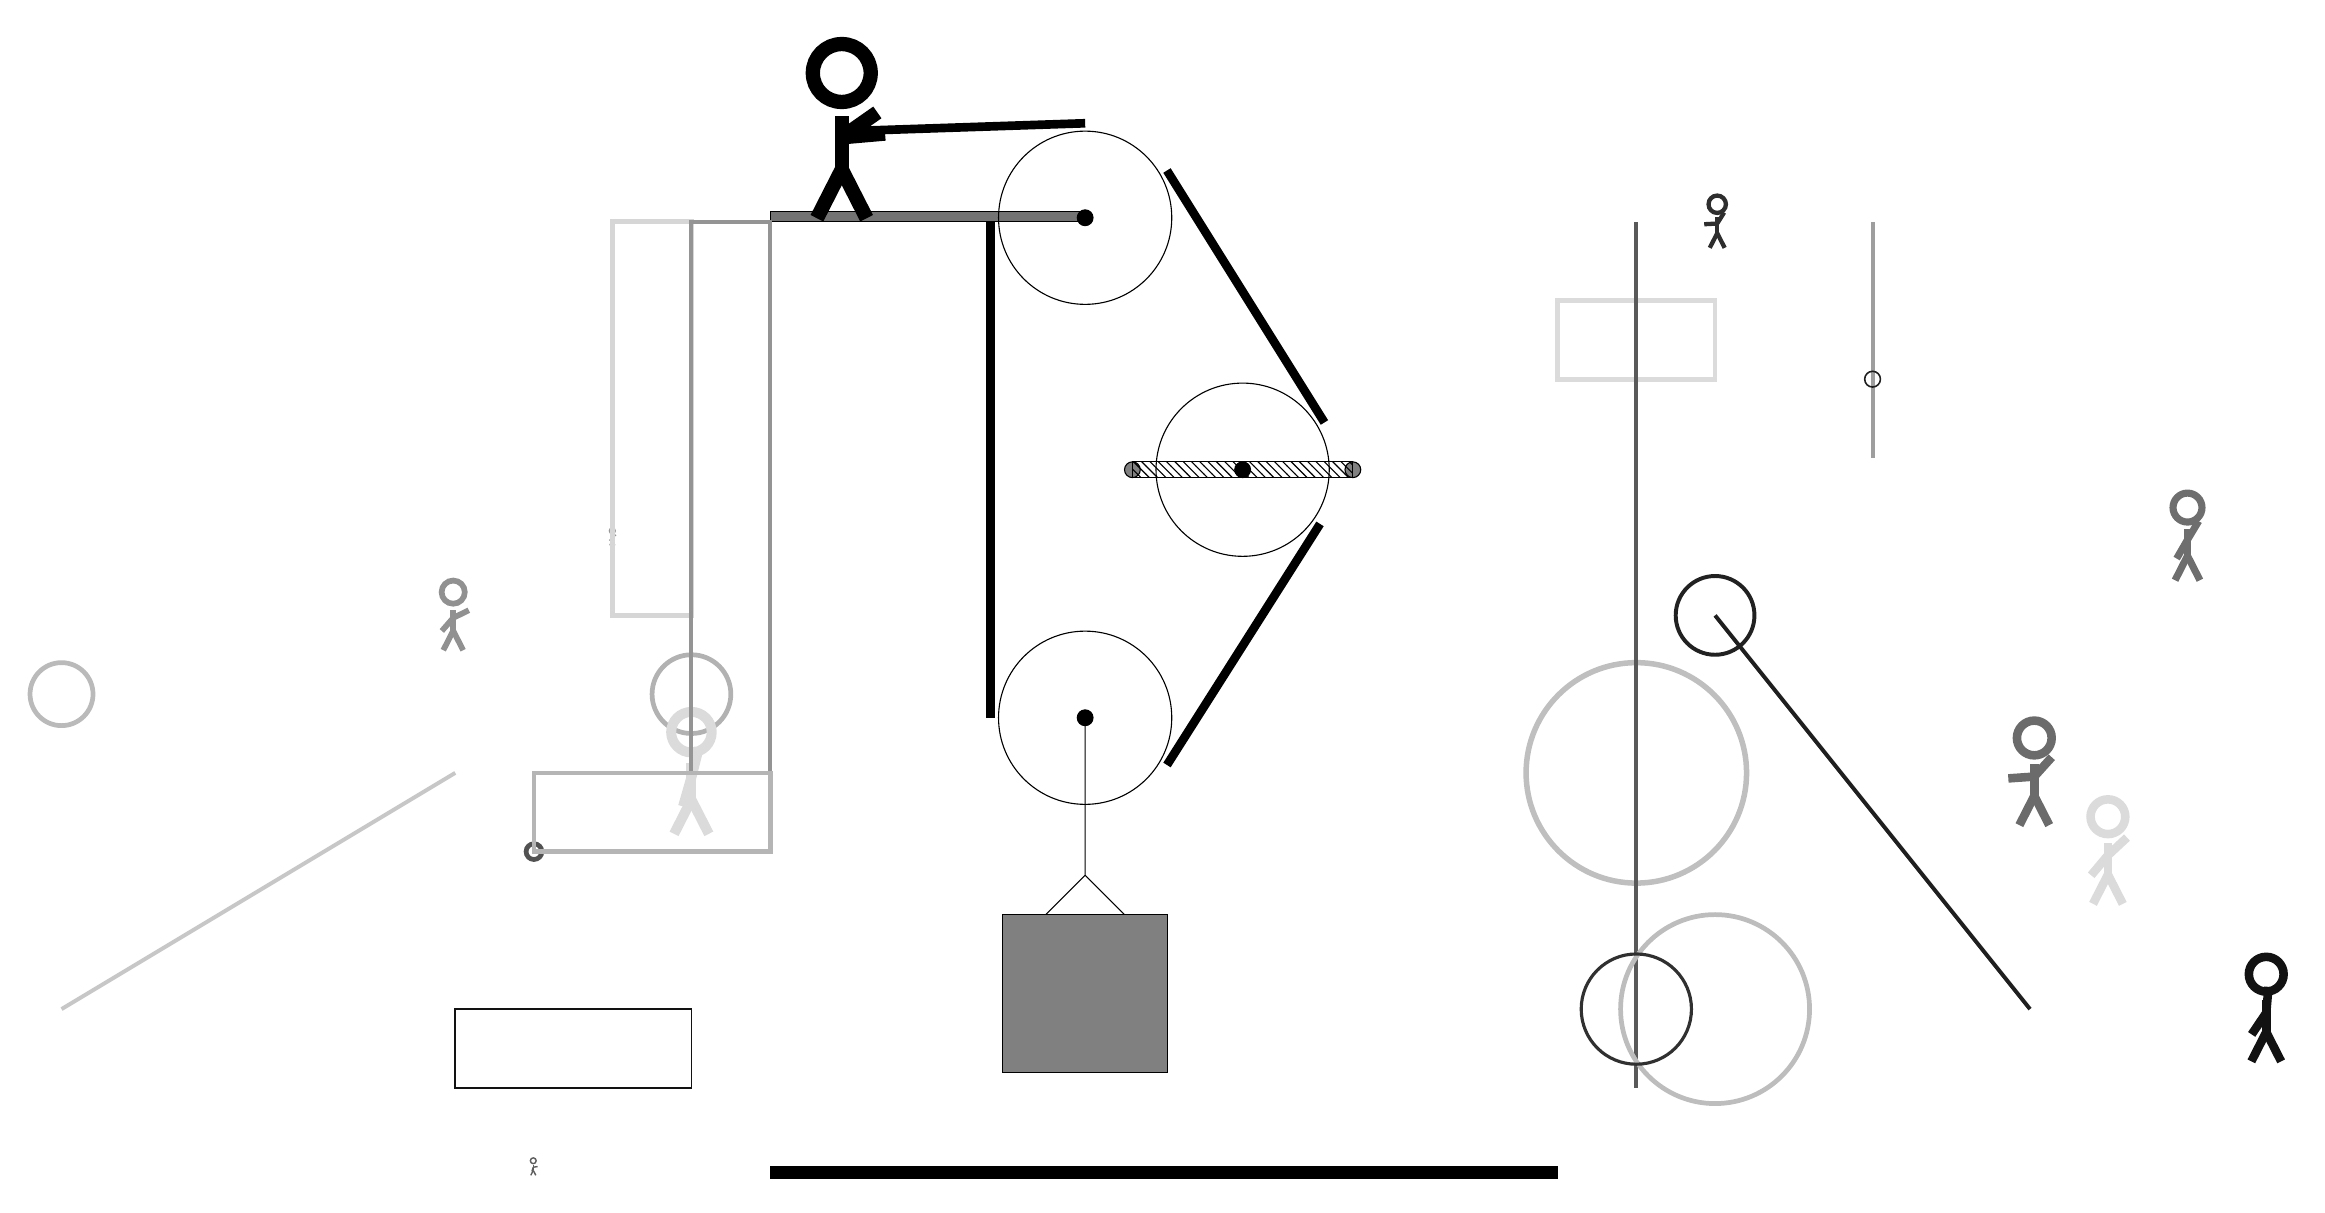
\begin{tikzpicture}
			%%%%% START %%%%%
			
			\draw[fill=black!55] (-2, 9) rectangle (2, 9.125);
			
			\draw (2, 2.7) circle (1.1);
			\draw[fill=black] (2, 2.7) circle (0.1);
			
			\draw (2, 9.05) circle (1.1);
			\draw[fill=black] (2, 9.05) circle (0.1);
			
			\draw[fill=white](4, 5.85) circle (1.1);
			\draw[fill=black] (4, 5.85) circle (0.1);
			\draw[fill=black!50] (2.6, 5.85) circle (0.1);
			\draw[fill=black!50] (5.4, 5.85) circle (0.1);
			\draw[pattern=north west lines, pattern color=black] (2.6, 5.95) rectangle (5.4, 5.75);
			
			\draw (2, 2.7) -- (2, 0.7) -- (1.5, 0.2) -- (2.5, 0.2) -- (2, 0.7);
			\draw[fill=black!50] (0.95, 0.2) rectangle (3.05, -1.8);
			
			\draw[line width=1.1mm] (0.8, 9) -- (0.8, 2.7);
			\centerarc[line width=1.1mm](2, 2.7)(180:330:1.2000000000000002);
			\draw[line width=1.1mm](3.0392, 2.1) -- (4.983, 5.1617);
			\centerarc[line width=1.1mm](4, 5.85)(390:325:1.2000000000000002);
			\draw[line width=1.1mm](5.0392, 6.45) -- (3.0392, 9.65);
			\centerarc[line width=1.1mm](2, 9.05)(30:90:1.2000000000000002);
			\draw[line width=1.1mm](2, 10.25) -- (-1, 10.15);
			
			\node[line width=0.2mm, color=black!93] at (17, -1) {\Strichmaxerl[6][56][85]};
			
			\draw[line width=0.6mm, color=black!14] (8, 8) rectangle (10, 7);
			\node[line width=0.4mm, color=black!82] at (10, 9) {\Strichmaxerl[3][3][58]};
			\draw [line width=0.5mm, color=black!87](10, 4) circle (0.5);
			\node[line width=0.3mm, color=black!63] at (-5, -3) {\Strichmaxerl[1][72][8]};
			
			\draw[line width=0.5mm, color=black!38](12, 6) -- (12, 9);
			\draw [line width=0.2mm, color=black!88](12, 7) circle (0.1);
			
			\draw [line width=0.6mm, color=black!68](-5, 1) circle (0.1);
			\draw[line width=0.5mm, color=black!88](10, 4) -- (14, -1);
			\node[line width=0.5mm, color=black!58] at (14, 2) {\Strichmaxerl[6][4][48]};
			\draw [line width=0.7mm, color=black!25](9, 2) circle (1.4);
			\draw [line width=0.6mm, color=black!30](-3, 3) circle (0.5);
			\node[line width=0.3mm, color=black!41] at (-4, 5) {\Strichmaxerl[1][50][32]};
			\draw[line width=0.6mm, color=black!16] (-4, 4) rectangle (-3, 9);
			\node[line width=0.6mm, color=black!57] at (16, 5) {\Strichmaxerl[5][60][59]};
			\draw[line width=0.5mm, color=black!65](9, -2) -- (9, 9);
			
			\node[line width=0.5mm, color=black!14] at (-3, 2) {\Strichmaxerl[7][74][76]};
			\draw[line width=0.5mm, color=black!42] (-3, 2) rectangle (-2, 9);
			\draw [line width=0.6mm, color=black!26](10, -1) circle (1.2);
			
			\node[line width=0.2mm, color=black!43] at (-6, 4) {\Strichmaxerl[4][49][26]};
			\node[line width=0.2mm, color=black!14] at (15, 1) {\Strichmaxerl[6][50][43]};
			
			\draw[line width=0.5mm, color=black!22](-6, 2) -- (-11, -1);
			\draw [line width=0.6mm, color=black!27](-11, 3) circle (0.4);
			\draw[line width=0.2mm, color=black!93] (-3, -1) rectangle (-6, -2);
			\draw[line width=0.6mm, color=black!29] (-2, 1) rectangle (-5, 2);
			\draw [line width=0.4mm, color=black!81](9, -1) circle (0.7);
			
			\node at (-1, 10.15) {\Strichmaxerl[10][-175][35]};
			
			\draw[fill=black] (-2, -3) rectangle (8, -3.15);
			
			%%%%% END %%%%%
		\end{tikzpicture}
	\end{figure}	
\end{document}